\chapter{推定に失敗したときの対策}\label{failure}

ここでは、最尤推定がうまくいかない場合の対処法についてまとめます。MNLモデルよりも高度なモデルを用いる場合、モデリングの誤りやバグが原因で推定が失敗することがあります。このような場合、どのようにデバッグを進めるべきかを図\ref{fig:estimation_failure}に示します。

\begin{figure}[ht]
    \centering
    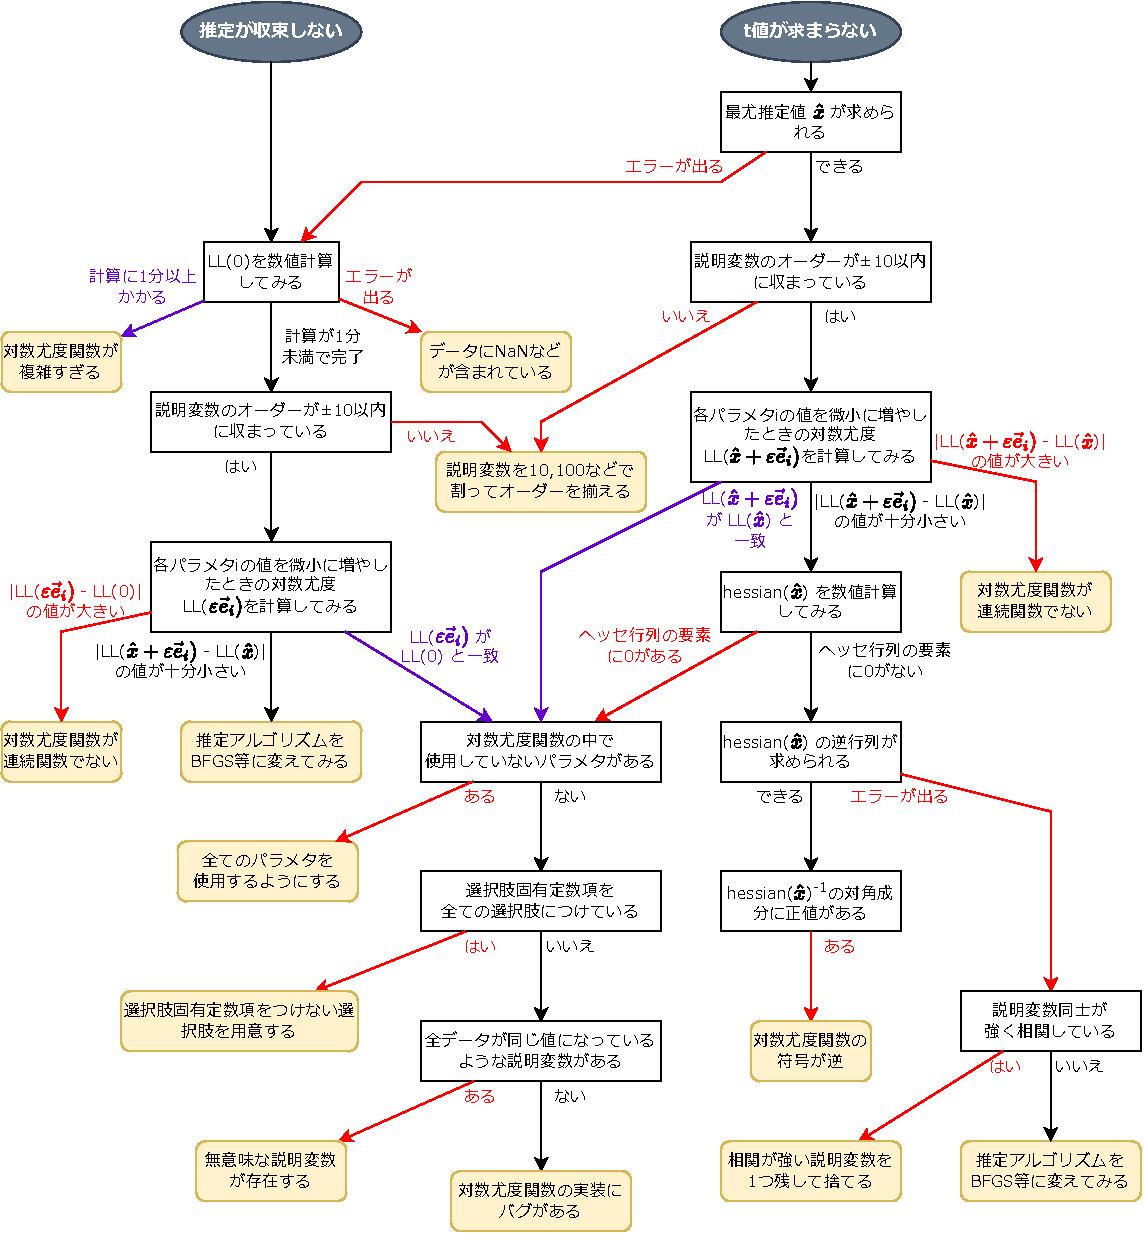
\includegraphics[width=0.95\hsize]{figure/estimation_failure.pdf}
    \caption{推定失敗時のデバッグフローチャート}
    \label{fig:estimation_failure}
\end{figure}

判断の根拠となる基準を示します。

\begin{description}
    \item[説明変数のオーダーが $\pm 10$ 以内に収まっていない] 説明変数の値が大きすぎると、数値計算の際にオーバーフローが発生する可能性があります。尤度関数の計算過程で $\exp(V)$ が出現するためです。例えば運賃(円)を説明変数に入れる場合は、データを $1/100$ 倍や $1/1000$ 倍にすることが望ましいです。
    \item[$LL(\hat x + \varepsilon e_i)=LL(\hat x)$] 対数尤度関数の勾配が消失していることを意味します。これは、対数尤度関数の値に影響を与えないパラメータが含まれていることを示しています。このようなパラメータを特定し、モデルから除外することで推定が可能になります。
    \item[$|LL(\hat x + \varepsilon e_i)-LL(\hat x)|$の値が大きい] 対数尤度関数の勾配が大きすぎる、またはそもそも連続でない場合が考えられます。この場合、最適化アルゴリズムが発散したり、hessianが異常な値を取ることがあります。このような場合は、モデルの再検討が必要です。
    \item[hessian($\hat x$)の逆行列が求められない] 正しく最尤推定値が求められていない可能性があります。ちなみに、ヘッセ行列が負定値行列ならば、尤度関数は極大値をとります。そして負定値行列は必ず逆行列を持ちます。逆に「極大値ならば負定値行列になる」とは限りませんが、多くの場合で成り立つので、逆行列が求められないということは推定値が極大値でない可能性があります。
    \item[hessian($\hat x$)の逆行列の対角成分に正の値が含まれる] 対数尤度関数の符号が間違っていると考えられます。負定値行列の逆行列は負定値行列なので、ヘッセ行列の逆行列の対角成分は通常負の値になるはずです。\ref{sec:code_likelihood_estimate}節での実装のように、最適化ライブラリの都合で符号を反転させている場合によくあるミスです。
\end{description}
